\subsection{Bereitstellung von Software}\label{bereitstellung}
Wurde der Bedarf einer neuen Software vom Fahrzeug festgestellt, muss diese im folgenden bereitgestellt werden. Zuvor muss der Softwarezulieferer die Sicherheit von Softwarepaketen verifizieren und eine sichere Kommunikation zwischen Servern und Fahrzeugen herstellen. Der Server muss alle vorhandenen Softwarepakete verwalten und auf Anfrage das am besten geeignete Softwarepaket für das jeweilige Fahrzeug identifizieren und ein Angebot an dieses schicken. Das Fahrzeug muss die eingegangen Softwareangebote über die Mensch-Maschine-Schnittstelle zu einem Zeitpunkt anbieten, an dem die Kaufbereitschaft des Fahrers möglichst hoch ist. Hierzu bedarf es einem Softwaremanagement, welches die Angebote des Servers verarbeitet. Da die Grundvoraussetzung der Wertschöpfungskette eine sichere Kommunikation zwischen Auto und Softwarelieferanten ist, wird zunächst eine mögliche Architektur zur sicheren Kommunikation vorgestellt.

\subsubsection{OTA-Aktualisierungen mit UPTANE}\label{3.1}\label{uptane}
Der im folgenden vorgestellte Standard "UPTANE", stellt eine Architektur und Vorgehensweise für die sichere Kommunikation zwischen einem Server und einem Auto 
vor. Hierdurch können Software-Aktualisierungen an intelligente Fahrzeuge sicher verteilt werden \cite{uptane}. Erste Schritte hierzu wurden 2010 getätigt, als Justin Samuel, Nick Mathewson, Roger Dingledine und Justin Cappos \textit{"The Update Framework" (TUF)} entwickelten. Dieses bildet den Grundbaustein für den späteren "\textbf{UPTANE}"-Standard. Mittlerweile ist es Teil des "Automotive Grade Linux Projekts" und somit Teil der "Linux Foundation". Uptane stellt mittels einer Mehrschichtenarchitektur sicher, dass im Rahmen von Aktualisierungen keine Schädlingssoftware auf ein Auto gelangt. Zunächst wird die Architektur von Uptane dargestellt(Abb. 4).

\begin{figure}[H]
  \begin{center}
    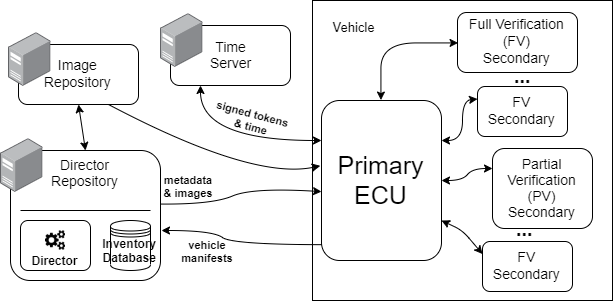
\includegraphics[width=0.95\textwidth]{../pictures/meta_model_fs-uptane-original.png}
  \end{center}
  \caption{Architektur Design UPTANE \cite{uptane}}
\end{figure}

Es ist vorab wichtig zu erwähnen, dass Uptane lediglich der Standard ist und keine offizielle Implementierung bereitstellt. Beispielhafte Implementierungen wären aktualizr\footnote{https://github.com/advancedtelematic/aktualizr},  rust-tuf\footnote{https://github.com/heartsucker/rust-tuf}, Notary\footnote{https://github.com/theupdateframework/notary} oder die OTA Dommunity Edition\footnote{https://github.com/advancedtelematic/ota-community-edition/}.
Kommerziell entwickelte Systeme werden bereitgestellt von HERE Technologies \footnote{https://www.here.com/products/automotive/ota-technology} sowie von   Airbiquity\footnote{https://www.airbiquity.com/product-offerings/software-and-data-management}.\\
Die rechte Seite des Bildes stellt das Fahrzeug dar, die Elemente zur linken die Repositories. Diese Repositories sind Server und sie haben alle eine eigene wichtige Aufgabe. Der Time-Server ist dafür da, um ECUs über die aktuelle Zeit zu informieren, da viele ECUs keine Uhr haben\cite{uptane}. Das Image Repository speichert jedes derzeit vom Lieferanten verteilte Image zusammen mit den Meta-Daten, welche zur Authentizität benötigt werden. Es nutzt Offline-Schlüssel um alle Metadaten zu "unterschreiben" bzw. zu verifizieren, was einen hohen Sicherheitsvorteil darstellt. Das Director Repository entscheidet abhängig von den übergebenen Informationen des Autos genau, welche Images an die ECUs verteilt werden müssen. Ein Auto hat mehrere ECUs, welche sich in Speicherplatzgröße, Stromverbrauch und Aufgabenbereich unterscheiden. Die \textit{Primary ECU} verwaltet und steuert die Installationen auf den anderen ECUs.\\

In dem ersten Schritt einer Aktualisierung schickt das Fahrzeug sein Manifest an das Director Repository. Dieses enthält Informationen darüber, welche Images aktuell auf dem Auto installiert sind. Das Director Repository entscheidet anhand dessen, welche Software auf dem Fahrzeug installiert/aktualisiert werden soll. Die Metadaten und die neuen Images werden zurück an die ECU geschickt. Hier findet zunächst eine Verifikation der neuen Images statt, bevor sie anschließend bei erfolgreichem Test installiert werden. Die Verifikation der ECUs kann entweder vollständig oder teilweise erfolgen. \textbf{Vollständig }heißt in diesem Kontext, dass die Größe der Software und die Hashes, welche die ECU über die Metadaten vom Director Repository erhält, identisch sind zu denen der Metadaten die vom Image Repository zur Verfügung gestellt werden. Bei der \textbf{teilweisen} Verifikation  muss lediglich die Signatur der Metadaten des Director Repositories mit der Signatur der Metadaten vom Image Repository übereinstimmen.
\subsubsection{Anpassung von UPTANE Architektur}
Damit die durch UPTANE bereitgestellte Architektur die Erkennung und Bereitstellung neuer Fahrumfänge unterstützt, muss diese dementsprechend angepasst werden, damit neben dem Aktualisieren bereits installierter Software auch das Installieren neuer Software möglich ist. Hierzu wird die Architektur von UPTANE erweitert und angepasst.\\

Damit das Director Repository nicht nur bestimmen kann, welche Software eine Aktualisierung benötigt, sondern auch welche auf dem Fahrzeug installiert werden muss um den Bedarf zu decken, braucht es eine geeignete Kommunikationsgrundlage. Hierzu soll das zuvor vorgestellte OpenSCENARIO XML-Speicherformat verwendet werden. Um die Suche nach neuer Software für das Directory Repository zu ermöglichen, wird das in Abbildung 5 dargestellte \textit{"Scenario Repository"} eingeführt. In diesem werden OpenSCENARIO-Dateien gespeichert, welche als Basis für die Suche nach Software dienen. Jede Datei hat hält mindestens \textbf{eine} Referenz in Form eines Schlüssels auf eine Software aus dem Image Repository.
\begin{figure}[H]
	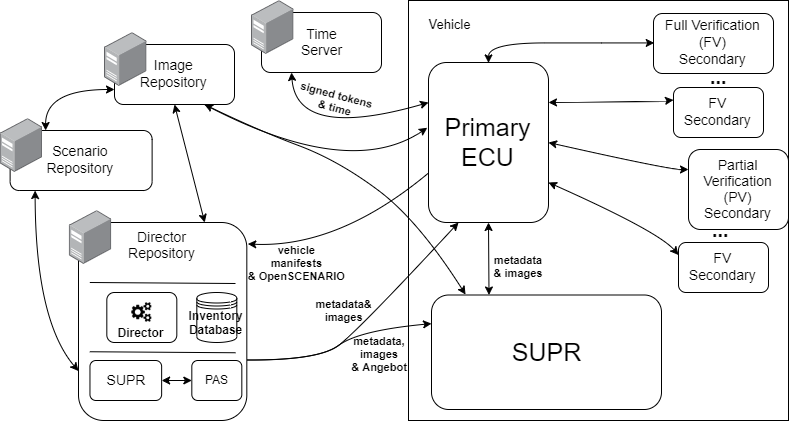
\includegraphics[width=0.95\textwidth]{../pictures/meta_model_fs-uptane-adjusted.png}
	\caption{Angepasste Uptane Architektur}
\end{figure}
Dies bedeutet, dass die jeweilige Situation der OpenScenario-Datei von eben dieser Software bewältigbar ist.  Erhält das Director Repository nun eine Anfrage für eine neue Software, wird diese anhand der mitgeschickten OpenSCENARIO-Dateien gesucht. Bei erfolgreicher Suche, soll diese in das Scenario Repository eingetragen werden. Die Suche führt der in Kapitel 2.3 eingeführte Software-User Pattern-Recognizer durch. In Kapitel 3.4 wird dieser um die Aspekte der Bereitstellung von Software erweitert.\\
Fahrzeughalter müssen neue Software kaufen, weshalb im Fall einer gefundenen Software zusätzlich zu den Metadaten und dem Softwarepaket \textit{(Softwareimage)} noch eine Sammlung verkaufsbezogener Daten verschickt werden muss. Diese wird hier und im folgenden \textbf{Angebot} genannt. Ein Angebot muss alle möglichen Verkaufsarten \textit{(Kauf, Miete, o.A.)} sowie dazu passende Preise beinhalten. Da die Preise und Verkaufsarten für Software je nach Automarke und -model variieren können sollen, wird ein Modul "pricing and sales", kurz PAS, zur Bestimmung des Preises und der Verkaufsart vorgeschlagen \textit{(siehe Abbildung 5)}. Das Director Repository ist nach wie vor dazu in der Lage, Softwareimages und Metadaten direkt an die Primäre Recheneinheit (ECU) zu schicken, wenn es sich nur um eine Aktualisierung bereits installierter Software handelt. Wird hingegen eine neue Software vorgeschlagen, so werden Image und Metadaten zusammen mit einem Angebot an den Software-User Pattern-Recognizer des Autos verschickt. Alternativ wird nur das Angebot verschickt um abzuwarten, ob der Kunde die Software tatsächlich haben will. Hierdurch würde das Image nicht unnötiger Weise verschickt werden, was unter anderem die Ressourcen schont. Der SUPR des Autos identifiziert unter stetiger Beobachtung des Fahrers, wann dieser einen Softwarevorschlag verarbeiten kann. Er stellt zum gegebenen Zeitpunkt Verbindung zu der Nutzeroberfläche des Wagens her, um so mit dem Fahrer zu kommunizieren und den Kaufvorgang abzuschließen \textit{(Ob erfolgreich oder nicht ist hierbei egal)}. Die Funktionsweisen und Aufgaben des SUPR im Auto unterscheiden sich von denen des SUPR im Director Repository. Aufgrund dessen ist es wichtig eine Abgrenzung und Spezifizierung dieser vorzunehmen.\\

\subsubsection{SUPR im Rahmen der Softwarebereitstellung}\label{3.3}
Das folgende komplettiert den in Kapitel 2.3 vorgestellten Software-User Pattern Recognizer \textit{(SUPR)}. Wie im ersten Teil wird auch im Rahmen der Bereitstellungskomponente des SUPR zwischen den Aufgaben auf Server und denen im Fahrzeug unterschieden.\\

\textbf{SUPR im Director Repository}\\
Die unterschiedlichen Suchvarianten welche der SUPR im Rahmen der Bedarfserkennung bereits auf dem Server ausführt, wurden in Kapitel 2.3 spezifiziert. Im Rahmen der Software Bereitstellung ist es die wesentliche Aufgabe, das Angebot und alle möglichen Preise festzulegen. Die verschiedenen Preise ergeben sich aus Kombination der einzelnen \textbf{Einflussfaktoren}.\\
Ein Angebot, welches vom Director Repository (siehe 3.2) an das SUPR des Fahrzeugs geschickt wird, spezifiziert die Preise für Software in Abhängigkeit der \textbf{Kaufart}, der \textbf{voraussichtlichen Laufzeit} des Mietverhältnisses (bei Miete), der Menge der Software welche der Fahrzeughalter in dem Moment akquirieren möchte und den eigentlichen Herstellungskosten der Software. Die folgende Tabelle definiert die Werte, welche die einzelnen Einflussfaktoren annehmen können.\\
\begin{center}
	\begin{tabularx}{\linewidth}{|p{2.8cm}|X|}
		\hline
		\textbf{Wert} & \textbf{Beschreibung}\\ [0.5ex] 
		\hline\hline
		\multicolumn{2}{|l|}{\textbf{Kaufart}}\\
		\hline
		Kauf & Der Fahrer akquiriert die Software dauerhaft. Eine Reklamation ist möglich, wenn diese ihre Aufgabe nicht korrekt ausführen würde.\\
		\hline
		Leihe & Der Fahrer legt einen Zeitraum\textit{(von .. bis)} fest, für welchen er diese Software akquirieren möchte. Für diesen bezahlt er im Voraus und die SW wird bei Ablauf des Zeitraums deinstalliert.\\
		\hline
		Miete/Abo & Der Fahrer wählt die Dauer einer Mietphase, an welche sich der Preis anpasst. Das Mietverhältnis wird nach Ablauf dieses Zeitraums aufrecht erhalten. Das heißt es entstehen laufend Kosten bis es vom Fahrer beendet wird.\\
		\hline
	\end{tabularx}
\end{center}
\begin{center}
	\begin{tabularx}{\linewidth}{|p{2.8cm}|X|}
		\hline
		\multicolumn{2}{|l|}{\textbf{Zeitraum/Dauer}}\\
		\hline
		Permanent & Der Zeitraum ist nur dauerhaft, wenn die Software gekauft wird. Hierbei tritt der höchste Preis auf.\\
		\hline
		Lang & Sechs Monate oder mehr. Auf einen Tag heruntergerechnet der günstigste Miet- oder Leihpreis.\\
		\hline
		Mittel & Sechs Wochen bis zu sechs Monate. Auf einen Tag heruntergerechnet ein wenig teurer als der des Langen.\\
		\hline
		Kurz & Acht Tage bis sechs Wochen. Auf einen Tag heruntergerechnet ein wenig teurer als der des Mittleren.\\
		\hline
		Einmalig & Ein bis sieben Tage. Auf einen Tag heruntergerechnet das teuerste Angebot.\\[0.5ex]
		\hline
	\end{tabularx}
\end{center}
\begin{center}
	\begin{tabularx}{\linewidth}{|p{2.8cm}|X|}
		\hline
		\multicolumn{2}{|l|}{\textbf{Menge}}\\
		\hline
		Einzeln & Es wird nur eine Software zu dem Zeitpunkt angeboten. Hat keinen Einfluss auf den Preis.\\
		\hline
		Mehrere & Software wird im Bundle gekauft, was sich positiv auf den Preis auswirkt. Ein Bundle muss vom SUPR im Fahrzeug erstellt werden.\\[0.5ex]
		\hline
		Flottenkauf & Es wird Software für mehrere Fahrzeuge gekauft. Dies kann für Unternehmen Sinnvoll sein, die Dienstwagen anbieten oder auch Autovermietungen etc.\\
		\hline 
	\end{tabularx}
\end{center}
\begin{center}
	\begin{tabularx}{\linewidth}{|p{2.8cm}|X|}
		\hline
		\multicolumn{2}{|l|}{\textbf{Weitere Einflüsse auf den Preis}}\\
		\hline
		Herstellungskosten & Die Kosten die im Laufe der (Weiter-)Entwicklung und der Wartung dieser Software entstanden sind. \\
		\hline
		Beliebtheit& Ist eine Software beliebt bzw. gefragt, steigt der Preis dieser. Die Beliebtheit kann entweder global gemessen werden oder regionsabhängig. Der Preisanstieg sollte dabei nicht zu hoch sein.\\
		\hline
		Mächtigkeit & Je mehr eine Software "kann", desto teurer sollte diese sein.\\
		\hline
	\end{tabularx}
\end{center}
Nachdem der SUPR des Director Repositorys eine den Bedarf deckende Software gefunden hat, muss er die Referenz auf die Datei an das PAS-Modul\textit{(siehe Abbildung)} schicken. Das PAS-Modul soll anhand der Software, einiger Informationen zum Kaufverhalten der Fahrer des Fahrzeugs sowie dem generellen Bedarf der Software ein personalisiertes \textit{Angebot} erstellen und anschließend an das Fahrzeug schicken.\\
\textbf{SUPR im Fahrzeug}\\
Neben dem Server-seitigen SUPR hat auch der SUPR des Autos wichtige Funktionen im Rahmen der Bereitstellung von Software. 
Ist das Angebot im Auto angekommen, identifiziert dieser einen geeigneten Verkaufszeitpunkt und stellt zu diesem das personalisierte Angebot über die Mensch-Maschine Schnittstelle (MMS)dar. Dies meint den Zeitpunkt, an dem der Verkauf oder die Leihe von Software möglichst wahrscheinlich ist. Hierzu ist eine Beobachtung des Fahrers nötig, um anhand von dessen \textbf{Eigenschaften} wie bspw. Mimik, Gestik, Sprache oder dem Fahrverhalten das Stress-, Freude, oder Angstlevel zu deuten, aber auch um Müdigkeit oder Ablenkung feststellen zu können. Vor allem Faktoren wie "Stress, Freude und Angst beeinflussen unsere Meinung und Entscheidung." Vgl. \cite[S.44]{Spindler2016}.
So wird eine Software eher nicht gekauft, wenn der Fahrer in eine stressige Verkehrssituation überblicken muss, zum Beispiel wenn es dicht benebelt ist und man zur Zeit in einer unbekannten Gegend Auto fährt. Hingegen beeinflusst Freude einen eher dazu, einen Kauf zu tätigen. Angst ist für den Anwendungsfall des Verteilens neuer Fahrfunktionen divers zu deuten. Wenn der Fahrer Angst vor der Strecke hat die vor ihm liegt, muss der SUPR dies anders bewerten als Angst die Aufgrund anderer Einflüsse entsteht. Diese Beobachtung entspricht der dritten Richtlinie Mensch-zentrierter autonomer Fahrzeuge nach Lex Fridman. \cite[S. 3]{b5} Nach der fünften Richtline Fridmans, soll ein Auto von dem Moment dem ersten Einsteigens des Fahrers auf diesen personalisiert werden.\cite[S. 5]{b5} So ist es Sinnvoll, würde der SUPR persönliche Eigenschaften in seine Entscheidungsfindung zum geeigneten Verkaufszeitpunkt einfließen lassen. \\

Ein System eines Fahrzeugs soll laut Fridman Daten-orientiert sein\cite[S. 3]{b5}. Das heißt, dass ein Fahrzeug aus den aufgenommenen Daten lernen soll. Fusioniert man die bei der Fahrerbeobachtung aufgenommene Daten mit Daten über den Verkaufserfolg, kann der SUPR aus seinen Handlungen lernen und sich so optimieren. Hierdurch werden mögliche den Kauf negativ beeinflussende Faktoren identifiziert (zB. Stress) und der Fahrer so besser kennengelernt. Die Kaufbereitschaft des Fahrers soll in Folge dessen möglichst oft korrekt eingeschätzt werden.\\

Ist der Zeitpunkt bzw. Zeitrahmen identifiziert, stellt der SUPR über die Mensch-Maschinen-Schnittstelle das personalisierte Angebot dar. Der dargestellte Inhalt wird maßgeblich beeinflusst von den Aspekten der Verkaufspsychologie. Um die wesentliche Aufgabe des SUPR \textit{(Beobachtung \& Kommunikation mit Fahrer, Vermarkten von Software)} Sinnvoll zu modellieren, werden die Einflussfaktoren für den dargestellten Inhalt der MMS anhand der Prinzipien der Verkaufspolitik nach Markus Reinke \cite{vkPsy} erläutert.\\

Um einen Kunden vom Erwerb eines Produkts zu überzeugen, muss diesem etwas angeboten werden wodurch ein offenes Bedürfnis befriedigt. Dazu muss herausgefunden werden, welches Produkt geeignet ist, damit es so anschließend angeboten werden kann. Wie der SUPR die Bedürfnisse von Fahrern identifiziert ist in Kapitel 2.3 nachzulesen. Was bei dem Anbieten einer Software beachtet werden muss, wird in diesem Kapitel abgehandelt.\\
Kunden sind unterteilbar in Plus-, Chancen- und Minus-Kunden.\cite[S. 10ff.]{vkPsy} Minus-Kunden werden ein Produkt von Beginn an nicht kaufen wollen, so gut der Erwerb auch gestaltet sein wird. Plus-Kunden werden ein Produkt voraussichtlich kaufen. Um die Chancen-Kunden von einem Erwerb zu überzeugen, werden im Absatz von Unternehmen diverse Prinzipien angewendet. Es kann also die Schlussfolgerung gezogen werden, dass so gut der SUPR seinen Fahrer auch kennt und wie gut Produkte den Bedarf auch abdecken, der Kunde dennoch nicht immer eine Software erwerben wird. Um die Anzahl an Käufern möglichst hoch zu halten, soll der persönliche Nutzen den die SW für den Kunden hat dargestellt werden. So kann die Situation simuliert und dargestellt werden, in welcher das Fahrzeug den Softwarebedarf festgestellt hat.\\
\label{angebotserstellung}
\begin{large}
	\textbf{Das Differenzprinzip}\cite[S. 19fff.]{vkPsy}\\
\end{large}
Nach dem Differenzprinzip sollen unterbewusste Reize gesetzt werden, die zum Erwerb leiten. Zum Beispiel wird mit der teuersten Variante des Produkts geworben, damit der Kunde bei näherem betrachten des Angebots die tieferen Preise, also ein "kleineres Übel", entdeckt und sich darüber erfreut. Dabei soll nicht die Frage \textbf{ob} der Kunde bei einem kaufen möchte, sondern \textbf{was} der Kunden von einem kaufen will.\\
Stellt der SUPR das Angebot dar, soll eine Mietfunktion im Fokus stehen, zudem deutlich gemacht werden. Die Option "Software Kaufen" ist kleiner darzustellen zusammen mit dem jeweiligen Preis. Um dem Kunden die Möglichkeit zu lassen die Software nicht zu erwerben, muss ein dezenter Knopf in der Nutzeroberfläche sein, welcher den Angebotsprozess beendet. Durch die Unauffälligkeit kann der Kunde zum Kauf gelenkt werden bzw. zu der Frage \textbf{was} man kaufen möchte, nicht \textbf{ob}. Um einen unterbewussten Reiz zu setzen, kann eine Karte dargestellt werden wie häufig die Software in der Umgebung installiert wurde. Dies sollte allerdings nur geschehen, wenn die Nachfrage tatsächlich auffällig hoch ist. Hiermit würde auch der Nachahmungseffekt abgedeckt werden\textit{ (weiter unten)}.\\

\begin{large}
	\textbf{Das Do-ut-des-Prinzip}\cite[S. 33fff.]{vkPsy} \\
\end{large}
Nach diesem Prinzip, wird "gegeben, damit du gibst". Der Kunde wird durch beispielsweise Gratis-Proben angelockt um zum Erwerb bewegt zu werden. Will er dennoch nichts kaufen, kann um Weiterempfehlung gebeten werden. Dieser Bitte wird der Kunde vrs. nachkommen, da er im Vorfeld etwas "gratis" erhalten hat. Die \textit{"Zwei Schritte vor, einer Zurück Taktik"} hierbei anzuwenden ist sinnvoll. Das heißt, dass dem Kunden zuerst die teuersten Produkte gezeigt werden, um ihn anschließend auch hier mit niedrigen Preisen anderer Produkte beeindrucken und halten zu können. Es sollte ist hierbei auch nicht das Ziel das teuerste Produkt zu verteilen, sondern das eigentliche Ziel ist eines mit tieferem Preis.\\
Der SUPR kann dieses Prinzip anwenden, in dem er dem Kunden zu neu erworbener Software eine Test-Version einer anderen Software "schenkt", welche nach einem bestimmten Zeitraum (4 Wochen) abläuft. Diese Software sollte einen bestehenden Bedarf der Kunden abdecken.\\

\begin{large}
	\textbf{Das Konsequenzprinzip}\\
\end{large}
Konsequenz im Handeln wird in den meisten Kulturen als eine positive Charaktereigenschaft gewertet, strahlt Sicherheit aus. Zudem schafft es Vertrauen bei Kunden. Konsequenz kann unter anderem mittels wenn-dann-Fragen ausgestrahlt werden, also "Wenn wir Ihnen XY bieten, kaufen Sie dann?" Der Kunde würde bei Erfüllung seines Bedarfs eher kaufen. Und da der von ihm benannte Bedarf abgedeckt ist, wird er so von einem frühen Commitment überzeugt. Es sollen die Wünsche und Prioritäten der Kunden erkannt werden und anschließend das Produkt mit Fokus auf diese beworben werden.\\
Dieses Prinzip sollte vor allem verwendet werden, um einen "Fuß in die Tür zu bekommen" und nicht um das teure Produkt zu verkaufen. Sinnvoll ist es, nach dem Motto "Kleinvieh macht auch Mist" zu verkaufen. Der SUPR tut dies zum einen indem er die Situation, in welcher der Bedarf festgestellt wurde, auf der MMS darstellt und den Kunden so erinnert. Wenn der Kunde noch gar keine oder nur wenig Software erworben hat, soll ihm immer die Möglichkeit einer kostenlose Probe-Woche geboten werden. Dies soll bis zu fünfmal geschehen, danach wird ohne weiteres keine Gratis Software mehr angeboten.\\

\begin{large}
	\textbf{Das Nutzen des Nachahmungseffekts}\cite[S. 67fff.]{vkPsy}\label{nachahmungseffekt}
\end{large}
\begin{center}
	\textit{"Der Mensch ist grundsätzlich ein Gemeinschaftswesen und achtet daher sehr darauf, was andere von ihm denken, sowohl in der breiten Öffentlichkeit als auch in seinem engen persönlichen Umfeld." - Markus Reinke (Vgl. )\cite[S. 67]{vkPsy} }\\
\end{center}
Dieses Verhalten, der sogenannte \textbf{Nachahmungseffekt}, kann durch das Einsetzen verschiedener Techniken provoziert werden. Bei der \textbf{\textit{Zeugenumlastung}} lässt sich der Kunde bestätigen, dass ihr Unternehmen und Produkt "gut" ist indem er von anderen positives darüber in Erfahrung bringt. Eine Variante, wie diese vom SUPR angewendet werden kann, wurde zuvor bereits dargestellt. Bei der \textbf{\textit{Referenztechnik}} werden die Stammkunden eines Unternehmens gebeten Empfehlungsschreiben zu erstellen mit welchen im folgenden geworben werden kann. Der SUPR kann hierzu ein Bewertungssystem einführen und Nutzer können die Bewertung anderer Fahrer lesen und sich so eine Meinung der Software einholen. Dabei ist es sinnvoll, einige vorgefertigte Antwort/Bewertungsmöglichkeiten selber zur Verfügung zu stellen. Eine dritte Technik ist das \textbf{\textit{Empfehlungsmarketing}}, bei welchem Kunden gebeten werden uns an Freunde und Verwandte weiter zu empfehlen. In den zeiten von Social Media bietet es sich an, eine "Teilen"-Funktion zur Verfügung zu stellen. Der Fahrer soll Teilen können, wie viele Kilometer er in welcher Zeit zurückgelegt hat, wie viele davon autonom bewältigt wurden und welche Softwarepakete genutzt wurden.\\

Um eine hohe Resonanz herzustellen, ist es sinnvoll dem Kunden ähnlich zu sein, sympathisch zu wirken, Lob \& Anerkennung zu verteilen als auch andere zu unterstützen. Da es ungewohnt ist, Lob oder anderes von einem Computer zu erhalten, der SUPR aber dennoch eine hohe Resonanz erzielen soll, sollte den Kunden eine Bezugsstelle gegeben werden. Eine Referenz aus der Wirtschaft hierzu stellt "Meet Olli" dar\cite{meetolli}. Olli ist das Maskottchen des UserInterfaces (UI)von "Local Motors" (LM). LM stellt einen autonom fahrenden Bus her, mit welchem die Insassen über eine UI interagieren können. Olli hat "nur" zwei Augen und einen Mund, stellt hierdurch aber einen vermenschlichten Bezugspunkt für den Fahrer und die Insassen dar und gewinnt so das Vertrauen der Insassen. \\

Darüber hinaus soll der Kunde nicht von den Angeboten "erschlagen" werden, sondern der SUPR muss diese dosiert vorlegen. Wenn der Kunde kein Interesse hat, ist dies zu respektieren und er soll damit nicht weiter konfrontiert werden. Der SUPR soll nur die tatsächlich benötigte Software bewerben - ein einmalig aufgetretener Bedarf fällt da nicht drunter \textit{(Die Ausnahme ist, der Kunde ist ein absoluter Plus-Kunde)}. Es muss genügend Werbung betrieben werden damit möglichst viel Software verkauft wird. "Klassische" Werbung auf der MMS ist nicht Sinnvoll, sondern eher Werbung in Form von Gratis-Proben von Software-Paketen. Nutzt der Fahrer eine dieser Proben und die SW kommt zum Einsatz, kann der SUPR den Fahrer über die MMS darüber in Kenntnis setzen, wodurch er vor Augen geführt bekommt, dass er diese Software braucht.

Ein Auto wird allerdings nicht nur von einer Person gefahren, sondern möglicherweise von mehreren Familienmitgliedern, Mitarbeitern oder anderen Mietern im Falle von Carsharing. Das SUPR muss dazu in der Lage sein, diese einzelnen Personen auseinanderhalten zu können um keine falschen Entscheidungen zu treffen.\\

Wird dem SUPR ein Softwarevorschlag mit Angebot zugeschickt, soll dieser bis das Angebot angezeigt werden kann, diese Software schon anfangen herunterzuladen. Dadurch kann die Software, wenn sie erworben wird, bereits während der Fahrt installiert werden, was den Verkauf schneller und Nutzerfreundlicher gestaltet.
\subsubsection{Die Mensch-Maschine-Schnittstelle}\label{MMS}
Die Mensch-Maschine-Schnittstelle ist das System, über welches der Fahrer und das Auto mit einander interagieren. Im Kontext intelligenter Fahrzeuge handelt es sich hierbei meist um einen Bildschirm, mitunter haben Fahrzeuge auch einen integrierten Sprachassistenten.\\

Das Bereitstellen neuer Fahrfunktionen schließt mit ein, dass ein Fahrzeug zum Zeitpunkt A selbstständig Fahren kann und zum Zeitpunkt B nicht. Zwischen diesen Zeitpunkten muss eine Übergabe der Fahraufgabe von dem Fahrzeug an den Fahrer erfolgen. Dabei soll der Fahrer des Fahrzeugs über die momentane Verkehrslage ausreichend in Kenntnis gesetzt werden, um während und nach der Übergabe der Fahraufgabe die Sicherheit zu wahren. Der Begriff ausreichend definiert sich dabei wie folgt:
\begin{center}
	\textbf{Die Inkenntnissetzung gilt als vollständig, wenn die Mensch-Maschine-Schnittstelle alle Prinzipien von S. Debernard et Al. \cite{b16} erfüllt.}\\
\end{center}
Das zu entwickelnde Display soll Nutzer-zentriert (User-Centered) entwickelt werden, um die Anforderungen möglichst vieler Nutzer erfüllen können und zusätzlich den Faktor der "Vermenschlichung" zu erhöhen. Die geschaffene transparente Straßenführung über das Display eines Fahrzeugs, soll zusätzlich durch Audio-Assistenten unterstützt werden. Die MMS wird so durch zu einem audiovisuellem System.\\
Die Schnittstelle soll sich sowohl visuell als auch auditiv an die im Fahrzeug sitzenden Personen anpassen. So kann zum Beispiel die Schriftgröße größer sein, wenn eine Person im Rentenalter das Fahrzeug betritt oder ähnliches. Mögliche Features der Personalisierung \textit{(z.B. größere Icons, dunkles Design)} werden mit Hilfe der Personas \ref{personas} in der Bachelorarbeit erarbeitet. Im generellen soll der Nutzer auf dem Display eine Simulation des eigenen Autos sehen zusammen mit zusätzlicher Information gemäß den Prinzipien nach Debernard et. Al. Das Design des User-Interfaces kann vom Fahrer angepasst werden, wobei die intuitive Bedienung sich nicht verschlechtern soll. Durch die Vermenschlichung des MMS, einer Transparenten Straßenführung, der Möglichkeit die Steuerung jederzeit zu übernehmen sowie der höflichen Kommunikation mit dem Fahrer, wird das Vertrauen des Fahrers zu dem Fahrzeug gefördert\cite{meetolli}, was den Kauf von Software wahrscheinlicher macht. 
